\textbf{Phần 1. Trắc nghiệm lựa chọn (Học sinh quan sát hình và chọn đáp án đúng)}
\setcounterpageref{ex}{0}

% --- CÂU 1 ---
\begin{ex} %[1D1N01]
Quan sát tranh và cho biết có bao nhiêu chú chim đang đậu trên cành cây?
\begin{center}
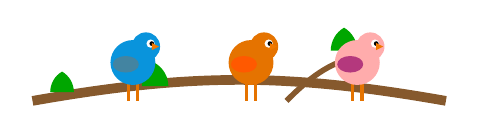
\begin{tikzpicture}[scale=0.75, baseline=(current bounding box.center)]
  % Cành cây
  \draw[line width=3.5pt, brown!70!black] (-3.5,-0.2) to[out=10,in=170] (3.5,-0.2);
  \draw[line width=2pt, brown!70!black] (0.8,-0.2) to[out=45,in=190] (2.2,0.6);
  % Chiếc lá
  \fill[green!65!black] (-1.2,0.05) arc (0:60:0.45) arc (120:180:0.45) -- cycle;
  \fill[green!65!black] (2.0,0.65) arc (0:60:0.45) arc (120:180:0.45) -- cycle;
  \fill[green!65!black] (-2.8,-0.05) arc (0:60:0.4) arc (120:180:0.4) -- cycle;
  % 3 chú chim xinh xắn
  \foreach \x/\c/\wing in {-1.8/cyan!80!blue/cyan!60!black, 0.2/orange!90!black/orange!70!red, 2.0/pink!90!red/magenta!70!black} {
    % Chân chim
    \draw[line width=1.2pt, orange!90!black] (\x-0.08,0.1) -- (\x-0.08,-0.2);
    \draw[line width=1.2pt, orange!90!black] (\x+0.08,0.1) -- (\x+0.08,-0.2);
    % Thân chim
    \fill[\c] (\x,0.45) circle (0.38cm);
    % Cánh chim
    \fill[\wing] (\x-0.12,0.42) ellipse (0.22cm and 0.14cm);
    % Đầu chim
    \fill[\c] (\x+0.22,0.72) circle (0.24cm);
    % Mắt chim
    \fill[white] (\x+0.3,0.77) circle (0.07cm);
    \fill[black] (\x+0.32,0.77) circle (0.04cm);
    % Mỏ chim
    \fill[orange!95!black] (\x+0.44,0.72) -- (\x+0.32,0.66) -- (\x+0.32,0.78) -- cycle;
  }
\end{tikzpicture}
\end{center}
\choice
{$2$}
{$4$}
{$5$}
{\True $3$}
\loigiai{
Đếm lần lượt từng chú chim đậu trên cành: có $1, 2, 3$ chú chim.\\
Số tương ứng là số $3$.\\
\textbf{Đáp án của câu hỏi là D}
}
\end{ex}

% --- CÂU 2 ---
\begin{ex} %[1D1N01]
Trong đĩa không có quả táo nào. Số quả táo trong chiếc đĩa tương ứng với chữ số nào?
\begin{center}
\begin{tikzpicture}[scale=0.8, baseline=(current bounding box.center)]
  % Chiếc đĩa tròn trống
  \draw[fill=cyan!10, draw=cyan!60!blue, line width=1.5pt] (0,0) ellipse (2.6cm and 0.8cm);
  \draw[fill=white, draw=cyan!40, line width=1pt] (0,-0.1) ellipse (2.1cm and 0.55cm);
  \node[font=\small\bfseries\itshape, text=gray!80!black] at (0,-0.1) {(Đĩa trống)};
\end{tikzpicture}
\end{center}
\choice
{\True $0$}
{$1$}
{$2$}
{$3$}
\loigiai{
Trong đĩa hoàn toàn không có quả táo nào, nghĩa là có $0$ quả táo.\\
Số không được viết bằng chữ số là $0$.\\
\textbf{Đáp án của câu hỏi là A}
}
\end{ex}

% --- CÂU 3 ---
\begin{ex} %[1D1H01]
Đoàn tàu hỏa đang chạy theo thứ tự từ bé đến lớn. Toa tàu liền sau toa số $3$ mang số nào?
\begin{center}
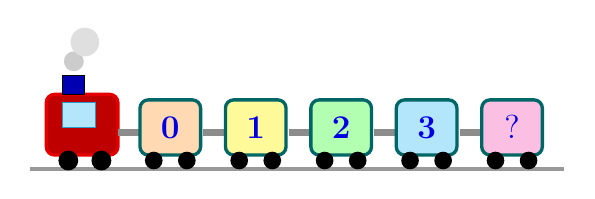
\begin{tikzpicture}[scale=0.7, baseline=(current bounding box.center)]
  % Đường ray
  \draw[line width=1.5pt, gray!80] (-4.5,-0.55) -- (5.2,-0.55);
  % Đầu tàu
  \draw[fill=red!75!black, draw=red!90!black, line width=1.2pt, rounded corners=3pt] (-4.2,-0.3) rectangle (-2.9,0.8);
  \draw[fill=cyan!30, draw=cyan!80!black] (-3.9,0.2) rectangle (-3.3,0.65); % cửa sổ đầu tàu
  \draw[fill=blue!70!black] (-3.9,0.8) rectangle (-3.5,1.15); % ống khói
  \fill[gray!40] (-3.7,1.4) circle (0.18);
  \fill[gray!25] (-3.5,1.75) circle (0.26);
  \fill[black] (-3.8,-0.4) circle (0.18); \fill[black] (-3.2,-0.4) circle (0.18);
  % Nối các toa
  \foreach \i/\num/\cl in {0/0/orange!30, 1/1/yellow!40, 2/2/green!30, 3/3/cyan!30, 4/{$\mathbf{?}$}/magenta!25} {
    \draw[line width=2.5pt, gray!90] (-2.9+\i*1.55,0.1) -- (-2.5+\i*1.55,0.1);
    \draw[fill=\cl, draw=teal!80!black, line width=1.2pt, rounded corners=3pt] (-2.5+\i*1.55,-0.3) rectangle (-1.4+\i*1.55,0.7);
    \node[font=\large\bfseries, text=blue!90!black] at (-1.95+\i*1.55, 0.2) {\num};
    \fill[black] (-2.25+\i*1.55,-0.4) circle (0.16);
    \fill[black] (-1.65+\i*1.55,-0.4) circle (0.16);
  }
\end{tikzpicture}
\end{center}
\choice
{$2$}
{\True $4$}
{$5$}
{$1$}
\loigiai{
Các số xếp theo thứ tự: $0, 1, 2, 3, 4, 5$.\\
Số đứng liền sau số $3$ là số $4$.\\
\textbf{Đáp án của câu hỏi là B}
}
\end{ex}

% --- CÂU 4 ---
\begin{ex} %[1D1H01]
Chú ếch nhảy qua các phiến lá sen mang số $0, \boxed{?}, 2, 3, 4, 5$. Chiếc lá sen đứng liền trước số $2$ mang số mấy?
\begin{center}
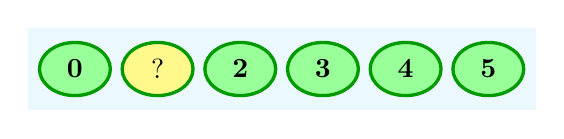
\begin{tikzpicture}[scale=0.75, baseline=(current bounding box.center)]
  % Mặt nước xanh
  \fill[cyan!8] (-0.8,-0.7) rectangle (7.8,0.7);
  % 6 phiến lá sen
  \foreach \x/\num/\col in {0/0/green!40, 1.4/{$\mathbf{?}$}/yellow!45, 2.8/2/green!40, 4.2/3/green!40, 5.6/4/green!40, 7.0/5/green!40} {
    \draw[fill=\col, draw=green!60!black, line width=1.2pt] (\x,0) ellipse (0.6cm and 0.45cm);
    \node[font=\bfseries\normalsize, text=black] at (\x,0) {\num};
  }
\end{tikzpicture}
\end{center}
\choice
{\True $1$}
{$0$}
{$3$}
{$4$}
\loigiai{
Đếm theo dãy số: $0, 1, 2, 3, 4, 5$.\\
Số đứng liền trước số $2$ là số $1$.\\
\textbf{Đáp án của câu hỏi là A}
}
\end{ex}

% --- CÂU 5 ---
\begin{ex} %[1D1H01]
Ba bạn gấu cầm các quả bóng bay mang số $2$, $\boxed{?}$, $4$. Quả bóng bay ở giữa mang số nào?
\begin{center}
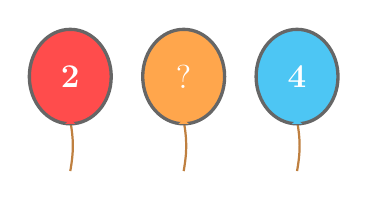
\begin{tikzpicture}[scale=0.8, baseline=(current bounding box.center)]
  \foreach \x/\num/\c in {-1.8/2/red!70, 0/{$\mathbf{?}$}/orange!70, 1.8/4/cyan!70} {
    % Dây bóng
    \draw[line width=0.8pt, brown] (\x,-1.0) to[out=80,in=-80] (\x,-0.2);
    % Quả bóng bay
    \draw[fill=\c, draw=black!60, line width=1.2pt] (\x,0.5) ellipse (0.65cm and 0.75cm);
    \fill[\c] (\x-0.08,-0.25) -- (\x+0.08,-0.25) -- (\x,-0.18) -- cycle;
    \node[font=\large\bfseries, text=white] at (\x,0.5) {\num};
  }
\end{tikzpicture}
\end{center}
\choice
{$1$}
{$5$}
{$0$}
{\True $3$}
\loigiai{
Dãy số liên tiếp: $2, 3, 4$.\\
Số đứng ở giữa số $2$ và số $4$ là số $3$.\\
\textbf{Đáp án của câu hỏi là D}
}
\end{ex}

% --- CÂU 6 ---
\begin{ex} %[1D1H01]
Dãy thẻ số nào dưới đây được xếp theo thứ tự từ bé đến lớn?
\begin{center}
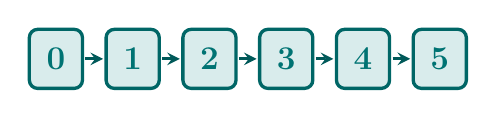
\begin{tikzpicture}[scale=0.75, baseline=(current bounding box.center)]
  \foreach \i/\num in {0/0, 1/1, 2/2, 3/3, 4/4, 5/5} {
    \draw[fill=teal!15, draw=teal!80!black, line width=1.2pt, rounded corners=3pt] (\i*1.3,-0.4) rectangle (\i*1.3+0.9,0.6);
    \node[font=\large\bfseries, text=teal!90!black] at (\i*1.3+0.45, 0.1) {\num};
    \ifnum\i<5
      \draw[->, >=stealth, line width=1pt, teal!70!black] (\i*1.3+0.95,0.1) -- (\i*1.3+1.25,0.1);
    \fi
  }
\end{tikzpicture}
\end{center}
\choice
{$5, 4, 3, 2, 1, 0$}
{\True $0, 1, 2, 3, 4, 5$}
{$1, 3, 2, 4, 5, 0$}
{$0, 2, 1, 3, 5, 4$}
\loigiai{
Dãy số đúng từ bé đến lớn bắt đầu từ số 0 là: $0, 1, 2, 3, 4, 5$.\\
\textbf{Đáp án của câu hỏi là B}
}
\end{ex}

% --- CÂU 7 ---
\begin{ex} %[1D1V01]
Đếm số ngón tay đang xòe ra ở bàn tay dưới đây:
\begin{center}
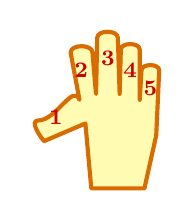
\begin{tikzpicture}[scale=0.75, baseline=(current bounding box.center)]
  % Bàn tay xòe 5 ngón
  \draw[fill=yellow!30, draw=orange!85!black, line width=1.5pt, line join=round]
    (0,-0.6) -- (-0.1,0.5) 
    -- (-0.8,0.2) to[out=130,in=180] (-0.9,0.55) to[out=0,in=110] (-0.2,0.9) % ngón cái
    -- (-0.35,1.7) to[out=90,in=90] (0.02,1.7) -- (0.08,1.0) % ngón trỏ
    -- (0.1,1.95) to[out=90,in=90] (0.45,1.95) -- (0.48,1.0) % ngón giữa
    -- (0.5,1.75) to[out=90,in=90] (0.82,1.75) -- (0.82,0.9) % ngón áp út
    -- (0.85,1.4) to[out=90,in=90] (1.15,1.4) -- (1.1,0.3) % ngón út
    -- (0.9,-0.6) -- cycle;
  % Đánh số ngón tay
  \node[font=\footnotesize\bfseries, text=red!80!black] at (-0.6,0.6) {1};
  \node[font=\footnotesize\bfseries, text=red!80!black] at (-0.17,1.4) {2};
  \node[font=\footnotesize\bfseries, text=red!80!black] at (0.28,1.6) {3};
  \node[font=\footnotesize\bfseries, text=red!80!black] at (0.66,1.4) {4};
  \node[font=\footnotesize\bfseries, text=red!80!black] at (1.0,1.1) {5};
\end{tikzpicture}
\end{center}
\choice
{\True $5$ ngón}
{$4$ ngón}
{$3$ ngón}
{$6$ ngón}
\loigiai{
Đếm lần lượt từng ngón tay: có đúng $5$ ngón tay.\\
\textbf{Đáp án của câu hỏi là A}
}
\end{ex}

% --- CÂU 8 ---
\begin{ex} %[1D1V01]
Có bao nhiêu chú cá đang tung tăng bơi lội trong bình cá?
\begin{center}

\begin{tikzpicture}[scale=0.8, baseline=(current bounding box.center)]
  % Bình cá tròn
  \draw[fill=cyan!15, draw=cyan!80!blue, line width=1.8pt] (0,0) circle (1.8cm);
  % Mặt nước uốn lượn
  \fill[cyan!35] (-1.75,-0.2) to[out=20,in=160] (1.75,-0.2) arc (0:-180:1.75cm) -- cycle;
  % Cây thủy sinh
  \draw[green!65!black, line width=2pt] (-0.9,-1.5) to[out=80,in=-80] (-0.7,-0.5);
  \draw[green!65!black, line width=2pt] (0.9,-1.5) to[out=100,in=-100] (0.7,-0.4);
  % 4 chú cá xinh
  \foreach \px/\py/\c in {-0.6/-0.6/orange, 0.5/-0.9/red, -0.2/-0.1/yellow!80!orange, 0.6/-0.2/orange!80!red} {
    \begin{scope}[shift={(\px,\py)}, scale=0.45]
      \fill[\c] (0,0) ellipse (0.42cm and 0.22cm);
      \fill[\c] (-0.38,0) -- (-0.65,0.22) -- (-0.65,-0.22) -- cycle; % đuôi cá
      \fill[white] (0.22,0.06) circle (0.07cm);
      \fill[black] (0.24,0.06) circle (0.04cm);
    \end{scope}
  }
\end{tikzpicture}
\end{center}
\choice
{$3$ chú cá}
{$5$ chú cá}
{\True $4$ chú cá}
{$2$ chú cá}
\loigiai{
Đếm trong bình: có $1, 2, 3, 4$ chú cá đang bơi.\\
Số lượng chú cá là $4$.\\
\textbf{Đáp án của câu hỏi là C}
}
\end{ex}

% --- CÂU 9 ---
\begin{ex} %[1D1V01]
Lan có $2$ cái bút chì màu vàng, mẹ cho Lan thêm $2$ cái bút chì màu xanh. Đếm tất cả có bao nhiêu cái bút chì?
\begin{center}
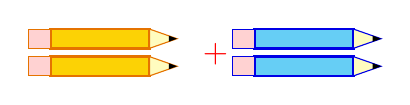
\begin{tikzpicture}[scale=0.7, baseline=(current bounding box.center)]
  % Nhóm 2 bút vàng
  \foreach \y in {0.5, 0} {
    \draw[fill=yellow!70!orange, draw=orange!90!black, line width=1pt] (-3,\y) rectangle (-1.2,\y+0.35);
    \draw[fill=pink!70, draw=orange!90!black] (-3.4,\y) rectangle (-3,\y+0.35); % tẩy
    \draw[fill=yellow!25, draw=orange!90!black] (-1.2,\y) -- (-0.7,\y+0.175) -- (-1.2,\y+0.35) -- cycle;
    \fill[black] (-0.85,\y+0.12) -- (-0.7,\y+0.175) -- (-0.85,\y+0.23) -- cycle;
  }
  \node[font=\large\bfseries, text=red] at (0,0.4) {$+$};
  % Nhóm 2 bút xanh
  \foreach \y in {0.5, 0} {
    \draw[fill=cyan!60, draw=blue!90!black, line width=1pt] (0.7,\y) rectangle (2.5,\y+0.35);
    \draw[fill=pink!70, draw=blue!90!black] (0.3,\y) rectangle (0.7,\y+0.35); % tẩy
    \draw[fill=yellow!25, draw=blue!90!black] (2.5,\y) -- (3.0,\y+0.175) -- (2.5,\y+0.35) -- cycle;
    \fill[black] (2.85,\y+0.12) -- (3.0,\y+0.175) -- (2.85,\y+0.23) -- cycle;
  }
\end{tikzpicture}
\end{center}
\choice
{$3$ cái}
{$5$ cái}
{\True $4$ cái}
{$2$ cái}
\loigiai{
Đếm tất cả số bút chì: $2$ cái bút vàng và $2$ cái bút xanh là $4$ cái bút chì.\\
\textbf{Đáp án của câu hỏi là C}
}
\end{ex}

% --- CÂU 10 ---
\begin{ex} %[1D1V01]
Trong chùm bóng bay mang số $4, 2, 0, 5, 3$ dưới đây, quả bóng nào mang số \textbf{bé nhất}?
\begin{center}
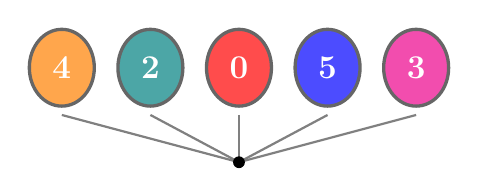
\begin{tikzpicture}[scale=0.75, baseline=(current bounding box.center)]
  \foreach \x/\num/\c in {-3/4/orange, -1.5/2/teal, 0/0/red, 1.5/5/blue, 3/3/magenta} {
    \draw[line width=0.8pt, gray] (\x,-0.8) -- (0,-1.6);
    \draw[fill=\c!70, draw=black!60, line width=1.2pt] (\x,0) ellipse (0.55cm and 0.65cm);
    \node[font=\large\bfseries, text=white] at (\x,0) {\num};
  }
  \fill[black] (0,-1.6) circle (0.1cm);
\end{tikzpicture}
\end{center}
\choice
{$2$}
{\True $0$}
{$3$}
{$4$}
\loigiai{
Trong các số $4, 2, 0, 5, 3$, số bé nhất là số $0$.\\
\textbf{Đáp án của câu hỏi là B}
}
\end{ex}

% --- CÂU 11 ---
\begin{ex} %[1D1V01]
Trong các ngôi sao mang số $1, 4, 3, 5, 2$, ngôi sao nào mang số \textbf{lớn nhất}?
\begin{center}
\begin{tikzpicture}[scale=0.75, baseline=(current bounding box.center)]
  \foreach \x/\num in {-3/1, -1.5/4, 0/3, 1.5/5, 3/2} {
    \node[draw=orange!80!black, fill=yellow!80, star, star points=5, star point ratio=2.2, line width=1.2pt, minimum size=1.1cm] at (\x,0) {};
    \node[font=\bfseries\normalsize, text=red!85!black] at (\x,-0.02) {\num};
  }
\end{tikzpicture}
\end{center}
\choice
{$4$}
{$3$}
{$1$}
{\True $5$}
\loigiai{
So sánh các số: $1 < 2 < 3 < 4 < 5$. Số lớn nhất là số $5$.\\
\textbf{Đáp án của câu hỏi là D}
}
\end{ex}

% --- CÂU 12 ---
\begin{ex} %[1D1C01]
Chú sâu đo ngộ nghĩnh có các đốt mang số: $0, 1, \dots, 3, 4, 5$. Số còn thiếu ở dấu $\mathbf{?}$ là số nào?
\begin{center}
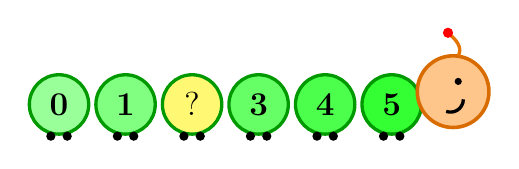
\begin{tikzpicture}[scale=0.65, baseline=(current bounding box.center)]
  \foreach \x/\num/\c in {0/0/green!40, 1.3/1/green!50, 2.6/{$\mathbf{?}$}/yellow!55, 3.9/3/green!60, 5.2/4/green!70, 6.5/5/green!80} {
    \draw[fill=\c, draw=green!60!black, line width=1.2pt] (\x,0) circle (0.58cm);
    \node[font=\large\bfseries, text=black] at (\x,0) {\num};
    \fill[black] (\x-0.16,-0.62) circle (0.09); \fill[black] (\x+0.16,-0.62) circle (0.09);
  }
  % Đầu sâu
  \draw[fill=orange!45, draw=orange!85!black, line width=1.3pt] (7.7,0.25) circle (0.7cm);
  \fill[black] (7.8,0.45) circle (0.07); % mắt
  \draw[line width=1.2pt] (7.9,0.1) arc (0:-110:0.25); % cười
  \draw[line width=1.2pt, orange!90!black] (7.8,0.95) to[out=60,in=-40] (7.6,1.4); % râu
  \fill[red] (7.6,1.4) circle (0.1);
\end{tikzpicture}
\end{center}
\choice
{$1$}
{$3$}
{\True $2$}
{$4$}
\loigiai{
Đếm dãy số từ $0$ đến $5$: $0, 1, 2, 3, 4, 5$.\\
Số còn thiếu ở giữa số 1 và số 3 là số $2$.\\
\textbf{Đáp án của câu hỏi là C}
}
\end{ex}

% =========================================================================
% PHẦN 2: TRẮC NGHIỆM ĐÚNG SAI (QUAN SÁT TRANH MINH HỌA)
% =========================================================================
\textbf{Phần 2. Trắc nghiệm đúng sai (Quan sát tranh và xét tính đúng/sai)}
\setcounterpageref{ex}{0}

% --- CÂU 13 ---
\begin{ex} %[1D1H01]
Quan sát tia số từ $0$ đến $5$ với các bước nhảy của chú cào cào:
\begin{center}
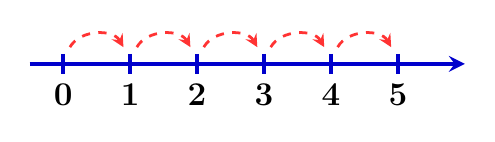
\begin{tikzpicture}[scale=0.85, baseline=(current bounding box.center)]
  % Tia số
  \draw[->, >=stealth, line width=1.5pt, blue!80!black] (-0.5,0) -- (6.0,0);
  \foreach \x in {0,1,2,3,4,5} {
    \draw[line width=1.5pt, blue!80!black] (\x,0.15) -- (\x,-0.15);
    \node[font=\bfseries\large, below] at (\x,-0.15) {\x};
  }
  % Các bước nhảy vòng cung
  \foreach \x in {0,1,2,3,4} {
    \draw[->, >=stealth, dashed, line width=1pt, red!80] (\x+0.1,0.25) to[out=60,in=120] (\x+0.9,0.25);
  }
\end{tikzpicture}
\end{center}
Xét tính đúng sai của các câu sau:
\choiceTF
{\True Số $0$ là số bé nhất trong các số từ $0$ đến $5$.}
{\True Số $5$ là số lớn nhất trong các số từ $0$ đến $5$.}
{Số $3$ đứng liền sau số $4$.}
{\True Số $3$ đứng liền trước số $4$.}
\loigiai{
\begin{itemize}
    \item Số $0$ ở vị trí đầu tiên bên trái nên là số bé nhất: \textbf{Đúng}.
    \item Số $5$ ở vị trí ngoài cùng bên phải nên là số lớn nhất: \textbf{Đúng}.
    \item Số $3$ đứng trước số $4$, không phải đứng sau: \textbf{Sai}.
    \item Số $3$ đứng liền trước số $4$: \textbf{Đúng}.
\end{itemize}
}
\end{ex}

% --- CÂU 14 ---
\begin{ex} %[1D1V01]
Quan sát bức tranh nông trại có các nhóm đồ vật sau:
\begin{center}
\begin{tikzpicture}[scale=0.7, baseline=(current bounding box.center)]
  % Ô 1: 1 chú gà trống
  \draw[fill=yellow!15, draw=orange!70, line width=1pt, rounded corners=4pt] (-4.8,-1) rectangle (-2.2,1.2);
  \node[font=\small\bfseries, text=orange!90!black] at (-3.5,0.9) {Gà trống};
  \fill[orange!90!black] (-3.5,0) circle (0.35cm);
  \fill[red] (-3.4,0.3) circle (0.15cm); % mào
  \node[font=\bfseries] at (-3.5,-0.6) {1 con};

  % Ô 2: 3 quả táo
  \draw[fill=red!10, draw=red!70, line width=1pt, rounded corners=4pt] (-1.8,-1) rectangle (1.2,1.2);
  \node[font=\small\bfseries, text=red!90!black] at (-0.3,0.9) {Quả táo};
  \foreach \x in {-1.0, -0.3, 0.4} {
    \fill[red!80!black] (\x,0) circle (0.28cm);
    \fill[green!70!black] (\x,0.28) circle (0.08cm);
  }
  \node[font=\bfseries] at (-0.3,-0.6) {3 quả};

  % Ô 3: 5 bông hoa
  \draw[fill=pink!15, draw=magenta!70, line width=1pt, rounded corners=4pt] (1.6,-1) rectangle (5.2,1.2);
  \node[font=\small\bfseries, text=magenta!90!black] at (3.4,0.9) {Bông hoa};
  \foreach \x in {2.1, 2.75, 3.4, 4.05, 4.7} {
    \fill[magenta!70] (\x,0.05) circle (0.22cm);
    \fill[yellow] (\x,0.05) circle (0.1cm);
  }
  \node[font=\bfseries] at (3.4,-0.6) {5 bông};
\end{tikzpicture}
\end{center}
Xét tính đúng sai của các câu sau:
\choiceTF
{\True Số lượng gà trống là $1$ con.}
{\True Số quả táo là $3$ quả.}
{Số quả táo nhiều hơn số bông hoa.}
{\True Nhóm bông hoa có số lượng nhiều nhất ($5$ bông).}
\loigiai{
\begin{itemize}
    \item Có $1$ chú gà trống: \textbf{Đúng}.
    \item Có $3$ quả táo: \textbf{Đúng}.
    \item $3$ quả táo ít hơn $5$ bông hoa (nói nhiều hơn là sai): \textbf{Sai}.
    \item Nhóm bông hoa có 5 bông là nhiều nhất: \textbf{Đúng}.
\end{itemize}
}
\end{ex}

% =========================================================================
% PHẦN 3: TRẢ LỜI NGẮN (ĐIỀN SỐ THÍCH HỢP VÀO Ô TRỐNG)
% =========================================================================
\textbf{Phần 3. Trả lời ngắn (Quan sát hình vẽ và điền số thích hợp)}
\setcounterpageref{ex}{0}

% --- CÂU 15 ---
\begin{ex} %[1D1H01]
Đếm số quả dâu tây trên chiếc đĩa dưới đây:
\begin{center}
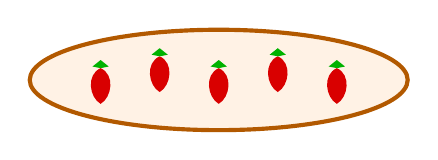
\begin{tikzpicture}[scale=0.75, baseline=(current bounding box.center)]
  % Chiếc đĩa
  \draw[fill=orange!10, draw=orange!70!black, line width=1.5pt] (0,-0.2) ellipse (3.2cm and 0.85cm);
  % 5 quả dâu tây
  \foreach \x/\y in {-2.0/0, -1.0/0.2, 0/0, 1.0/0.2, 2.0/0} {
    \begin{scope}[shift={(\x,\y)}, scale=0.55]
      \fill[red!85!black] (0,0) .. controls (-0.45,-0.2) and (-0.35,-0.9) .. (0,-1.1) .. controls (0.35,-0.9) and (0.45,-0.2) .. (0,0);
      \fill[green!70!black] (-0.25,0.05) -- (0,0) -- (0.25,0.05) -- (0,0.25) -- cycle;
    \end{scope}
  }
\end{tikzpicture}
\end{center}
\shortans{5}
\loigiai{
\textbf{Đáp số:} $5$\\
Đếm trên đĩa có $1, 2, 3, 4, 5$ quả dâu tây.
}
\end{ex}

% --- CÂU 16 ---
\begin{ex} %[1D1H01]
Quan sát sơ đồ tách - gộp số: Số $5$ gồm $3$ và mấy?
\begin{center}
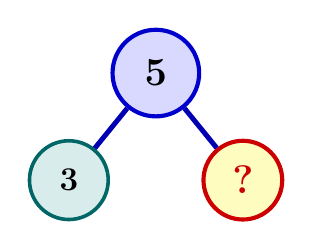
\begin{tikzpicture}[scale=0.85, baseline=(current bounding box.center)]
  % Quả to ở trên
  \node[draw=blue!80!black, circle, fill=blue!15, line width=1.5pt, minimum size=1.1cm, font=\bfseries\Large] (Tong) at (0,1.2) {5};
  % Hai nhánh ở dưới
  \node[draw=teal!80!black, circle, fill=teal!15, line width=1.3pt, minimum size=1cm, font=\bfseries\large] (N1) at (-1.3,-0.4) {3};
  \node[draw=red!80!black, circle, fill=yellow!25, line width=1.5pt, minimum size=1cm, font=\bfseries\Large, text=red!80!black] (N2) at (1.3,-0.4) {?};
  % Đường nối
  \draw[line width=1.8pt, blue!70!black] (Tong) -- (N1);
  \draw[line width=1.8pt, blue!70!black] (Tong) -- (N2);
\end{tikzpicture}
\end{center}
\shortans{2}
\loigiai{
\textbf{Đáp số:} $2$\\
Tách số: $5$ gồm $3$ và $2$.
}
\end{ex}

% --- CÂU 17 ---
\begin{ex} %[1D1V01]
Có bao nhiêu chiếc bánh kem thơm ngon trong hộp dưới đây?
\begin{center}
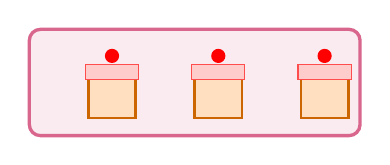
\begin{tikzpicture}[scale=0.75, baseline=(current bounding box.center)]
  \draw[fill=purple!8, draw=purple!60, line width=1.2pt, rounded corners=4pt] (-2.8,-0.8) rectangle (2.8,1.0);
  \foreach \x in {-1.8, 0, 1.8} {
    % Chiếc bánh
    \draw[fill=orange!25, draw=orange!80!black, line width=1pt] (\x,-0.5) rectangle (\x+0.8,0.2);
    \draw[fill=pink!80, draw=red!70] (\x-0.05,0.15) rectangle (\x+0.85,0.4);
    \fill[red] (\x+0.4,0.55) circle (0.12cm); % quả cherry
  }
\end{tikzpicture}
\end{center}
\shortans{3}
\loigiai{
\textbf{Đáp số:} $3$\\
Đếm trong hộp có đúng $3$ chiếc bánh kem.
}
\end{ex}

% --- CÂU 18 ---
\begin{ex} %[1D1V01]
Điền số còn thiếu vào chiếc lá sen có dấu $\mathbf{?}$:
\begin{center}
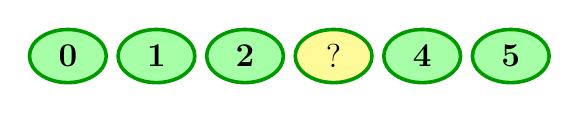
\begin{tikzpicture}[scale=0.75, baseline=(current bounding box.center)]
  \foreach \x/\num/\col in {0/0/green!35, 1.5/1/green!35, 3.0/2/green!35, 4.5/{$\mathbf{?}$}/yellow!40, 6.0/4/green!35, 7.5/5/green!35} {
    \draw[fill=\col, draw=green!60!black, line width=1.3pt] (\x,0) ellipse (0.65cm and 0.45cm);
    \node[font=\large\bfseries, text=black] at (\x,0) {\num};
  }
\end{tikzpicture}
\end{center}
\shortans{3}
\loigiai{
\textbf{Đáp số:} $3$\\
Thứ tự các số: $0, 1, 2, 3, 4, 5$. Số còn thiếu là $3$.
}
\end{ex}

% --- CÂU 19 ---
\begin{ex} %[1D1V01]
Có $3$ chú bướm tím đang bay lượn, có thêm $1$ chú bướm vàng bay tới. Hỏi có tất cả bao nhiêu chú bướm?
\begin{center}

\begin{tikzpicture}[scale=0.7, baseline=(current bounding box.center)]
  % 3 chú bướm tím
  \foreach \x/\y in {-3.2, -1.8, -0.4} {
    \begin{scope}[shift={(\x,0.2)}, scale=0.5]
      \fill[magenta!70!purple] (-0.2,0.2) ellipse (0.4 and 0.6);
      \fill[magenta!70!purple] (0.2,0.2) ellipse (0.4 and 0.6);
      \fill[pink!80] (-0.2,-0.3) ellipse (0.3 and 0.4);
      \fill[pink!80] (0.2,-0.3) ellipse (0.3 and 0.4);
      \fill[black] (0,0) ellipse (0.1 and 0.5);
    \end{scope}
  }
  \node[font=\Large\bfseries, text=red] at (0.8,0.2) {$+$};
  % 1 chú bướm vàng
  \begin{scope}[shift={(2.2,0.2)}, scale=0.5]
    \fill[yellow!90!orange] (-0.2,0.2) ellipse (0.4 and 0.6);
    \fill[yellow!90!orange] (0.2,0.2) ellipse (0.4 and 0.6);
    \fill[orange!80] (-0.2,-0.3) ellipse (0.3 and 0.4);
    \fill[orange!80] (0.2,-0.3) ellipse (0.3 and 0.4);
    \fill[black] (0,0) ellipse (0.1 and 0.5);
  \end{scope}
\end{tikzpicture}
\end{center}
\shortans{4}
\loigiai{
\textbf{Đáp số:} $4$\\
Gộp $3$ chú bướm và $1$ chú bướm là có tất cả $4$ chú bướm.
}
\end{ex}

% --- CÂU 20 ---
\begin{ex} %[1D1V01]
Trong chuồng không có chú gà nào. Hãy viết chữ số tương ứng với số chú gà trong chuồng:
\begin{center}
\begin{tikzpicture}[scale=0.75, baseline=(current bounding box.center)]
  % Hàng rào gỗ chuồng gà trống
  \draw[line width=3pt, brown!70!black] (-2.5,0.3) -- (2.5,0.3);
  \draw[line width=3pt, brown!70!black] (-2.5,-0.3) -- (2.5,-0.3);
  \foreach \x in {-2.0, -1.0, 0, 1.0, 2.0} {
    \draw[line width=4pt, brown!90!black] (\x,-0.6) -- (\x,0.7);
  }
  \node[font=\small\bfseries\itshape, text=gray!80!black] at (0,-1.0) {(Chuồng trống)};
\end{tikzpicture}
\end{center}
\shortans{0}
\loigiai{
\textbf{Đáp số:} $0$\\
Trong chuồng không có chú gà nào nghĩa là số $0$.
}
\end{ex}
